\section{Inserting the data}
\label{sec:inserting_the_data}

The purpose of the software is to create graphical representations of the
programs. The software suite works by merging independent information from
different courses. More specifically, the following items are required:
%
\begin{enumerate}
\item a \ac{KCM} (which is a specialized spreadsheet file) for each course;
\item a ``\emph{program definition file}'' (which is a plain text file) that
	indicates which \acp{KCM} are included in the program.
\end{enumerate}
%
This section goes over the procedure for creating the files above, and for
how to enter information in them.

\subsection{Creating the database containing the files above}
\label{creating_the_database}

The first step is to create a database containing the \ac{KCM} spreadsheets
and the program definition file. The \acp{KCM} may be in a remote location,
such as on Google Drive or Dropbox, or on the computer that runs this
software. The program definition file must be available on the computer,
regardless of where the \acp{KCM} are located.

\textbf{As for the program definition file}, it must be a tabulated list
structured as in Table~\ref{tab:progexample}. This means that the first row
\emph{must} be identical to that of the first row in
Table~\ref{tab:progexample}, where each column is separated by exactly one
tab. The other rows should each have a course code, a version number (any
positive rational number is valid) and a link to a \ac{KCM} on a remote
location (Google Drive, Dropbox, etc.), in order. Also here, each column has
to be separated by exactly one tab. 

\begin{table}[!htbp]
	\centering
	\caption{Example of a program definition file. Each column has to be
	separated by exactly one tab (this means that the columns may not
	look like ``aligned'' in the file).}
	\label{tab:progexample}
	\ttfamily
	\begin{tabular}[t]{lll}
		\toprule
			coursecode & version & link \\
		\midrule
			TX8101 & 2 & (URL link to the spreadsheet file) \\
			AF9101 & 3 & (URL link to the spreadsheet file) \\
			XY0011 & 2 & (URL link to the spreadsheet file) \\
		\bottomrule
	\end{tabular}
\end{table}

This file, let's call it \texttt{my-program-definition-file.txt}, should be
located in a specific path. To understand where, consider the base folder
shown and described in Figure~\ref{fig:file-structure-base-folder}.

\begin{figure}[!htbp]
	\centering
	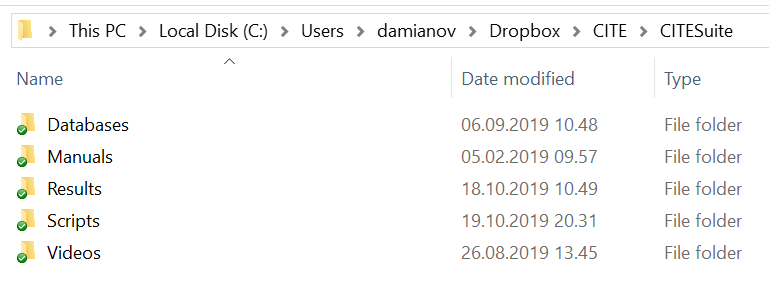
\includegraphics{file-structure-base-folder} 
	% TODO Get a new figure in place where it says ``COnCUR''.
	\caption{Structure of the base folder: when extracting the downloaded \texttt{COnCUR.zip} file, you obtain this.}
	\label{fig:file-structure-base-folder}
\end{figure}

From the base folder in Figure~\ref{fig:file-structure-base-folder}, enter
the ``Databases'' folder. The folder should be structured as in
Figure~\ref{fig:file-structure-databases-folder}.

\begin{figure}[!htbp]
	\centering
	% TODO Ibidem.
	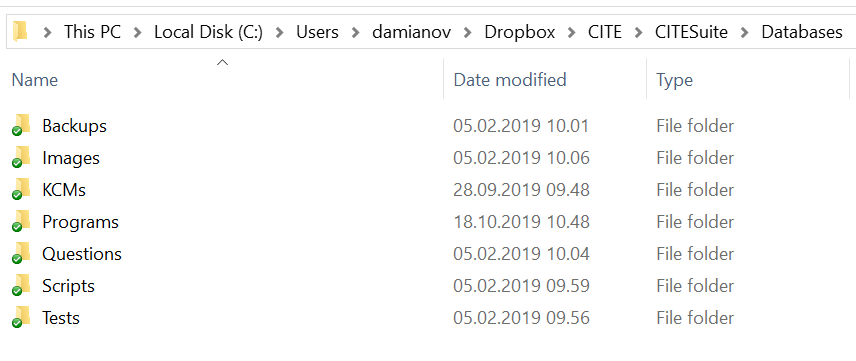
\includegraphics{file-structure-databases-folder}
	\caption{Structure of the ``databases'' folder.}
	\label{fig:file-structure-databases-folder}
\end{figure}

The \texttt{my-program-definition-file.txt} goes inside the folder
``Programs''. \textbf{As an example,} a person that has a few program
definition files may have a situation like in
Figure~\ref{fig:file-structure-programs-folder}.

\begin{figure}[!htbp]
	\centering
	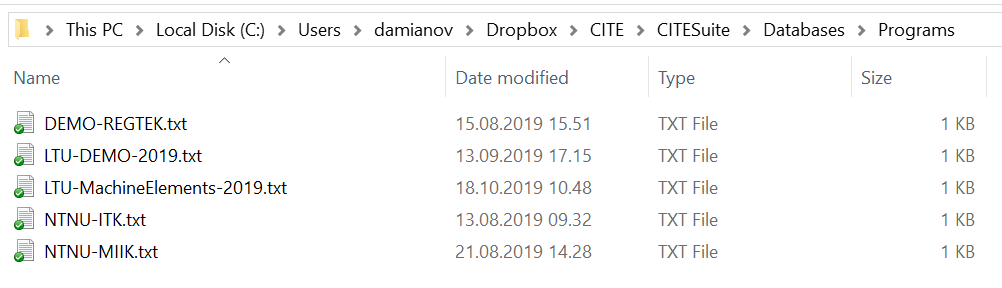
\includegraphics{file-structure-programs-folder}
	\caption{Example of how the ``Programs'' folder may look like. Note
	that when downloading the software suite you get an almost empty
	Programs folder (except a demo file).}
	\label{fig:file-structure-programs-folder}
\end{figure}

As for the \acp{KCM}, they can be either on the Internet or on a local
folder. Sections~\ref{sec:dbinternet}~and~\ref{sec:dblocal} explain how to
structure these.


\subsubsection{Internet-based case}
\label{sec:dbinternet}

One may want to keep the \ac{KCM} files on the Internet, so that different
persons may access and/or edit the information in an asynchronous way. The
program definition file tells where these are, and the software works by
downloading the \acp{KCM} when one runs the analysis. The structure of the
Internet-based database of the \acp{KCM} is as in
Figure~\ref{fig:dbinternet}.

\begin{figure}[!htbp]
	\centering
	\begin{tikzpicture}[auto]
		\node [block, name=root] {Databases};
		\node [block, name=programs, below right of=root] {Programs};
		\node [file, name=pfile, right of=programs] {\texttt{\textit{code}.txt}};
		\node [cloud, name=drive, right of=root] {Google Drive};
		\node [file, name=sheet1, right of=drive, node distance=10em] {\texttt{course1.xlsx}};
		\node [file, name=sheetN, below of=sheet1] {\texttt{courseN.xlsx}};
		
		\draw [draw] (root) -- (programs);
		\draw [draw, dotted] (root) -- (drive);
		\draw [draw] (programs) -- (pfile);
		\draw [draw] (drive) -- (sheet1);
		\draw [draw] (drive) -- (sheetN);
		\draw [draw, dashed] (sheet1) -- (sheetN);
	\end{tikzpicture}
	\caption{Diagram of the internet-based program database.}
	\label{fig:dbinternet}
\end{figure}

This means that the program definition file should be placed in the
\texttt{Programs} folder of the \texttt{Databases} folder, as said before,
and the links that it contains should point to the corresponding \acp{KCM}.

\subsubsection{Local repository case}
\label{sec:dblocal}

The other option is to have the \ac{KCM} files placed in suitable folders.
The structure of such a database is given in Figure~\ref{fig:dblocal}.

\begin{figure}[!htbp]
	\centering
	\begin{tikzpicture}[auto]
		\node [block, name=root] {Databases};
		\node [block, name=programs, below right of=root] {Programs};
		\node [file, name=pfile, right of=programs] {\texttt{\textit{code}.txt}};
		\node [block, name=kcms, right of=root] {KCMs};
		\node [block, name=drive, right of=kcms] {\textit{code}};
		\node [file, name=sheet1, right of=drive, node distance=10em] {\texttt{course1\_va.c.xlsx}};
		\node [file, name=sheetN, below of=sheet1] {\texttt{courseN\_vn.xlsx}};
		
		\draw [draw] (root) -- (programs);
		\draw [draw] (root) -- (kcms);
		\draw [draw] (kcms) -- (drive);
		\draw [draw] (programs) -- (pfile);
		\draw [draw] (drive) -- (sheet1);
		\draw [draw] (drive) -- (sheetN);
		\draw [draw, dashed] (sheet1) -- (sheetN);
	\end{tikzpicture}
	\caption{Diagram of the local database of the \ac{KCM} spreadsheet files.}
	\label{fig:dblocal}
\end{figure}

In more details, if one considers the base folder shown in
Figure~\ref{fig:file-structure-base-folder}, one should then enter the
Databases folder (as in Figure~\ref{fig:file-structure-databases-folder}),
and then enter the folder ``KCMs''. For a person that has been analysing
several programs, this ``KCMs'' folder would look like as in
Figure~\ref{fig:file-structure-KCMs-folder} (again, this is an example --
you get an almost empty ``KCMs'' folder when you download the software
suite).

\begin{figure}[!htbp]
	\centering
	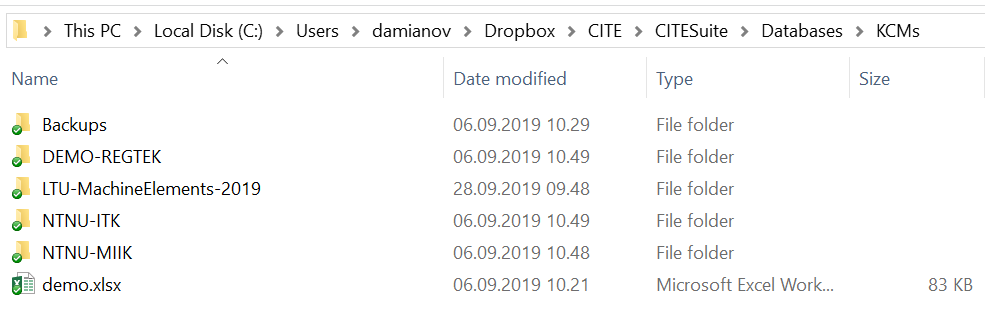
\includegraphics{file-structure-KCMs-folder}
	\caption{Structure of the ``KCMs'' folder for a person that has been analysing several programs.}
	\label{fig:file-structure-KCMs-folder}
\end{figure}

Each folder in the ``KCMs'' folder is then a separate program: in this
sub-folder you shall place your \texttt{.xlsx} files. As an example,
Figure~\ref{fig:file-structure-NTNU-MIIK-folder} shows the content of such a
sub-folder relative to a program in NTNU. Note that one may have different
versions for the same course. Note also that if a \ac{KCM} is not found, the
program will download it from the Internet and copy the downloaded sheet to
its expected location.

\begin{figure}[!htbp]
	\centering
	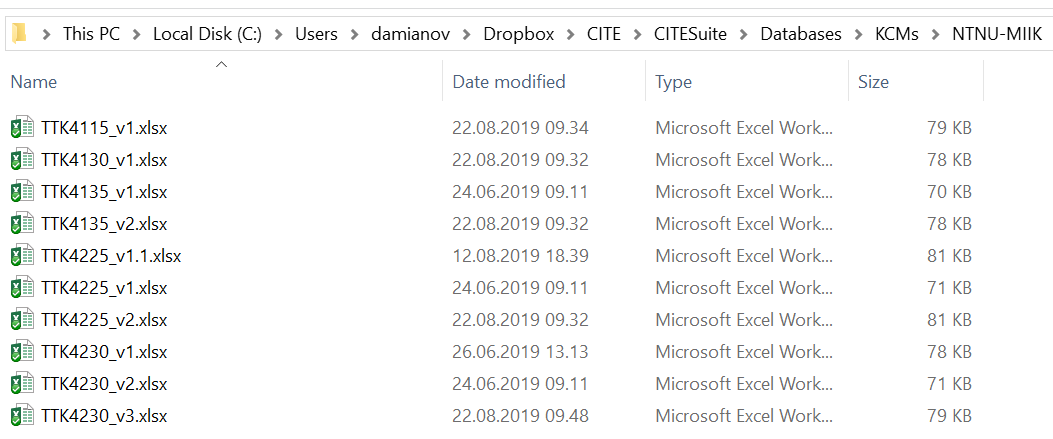
\includegraphics{file-structure-NTNU-MIIK-folder}
	\caption{Contents of a folder that contains the \texttt{.xlsx} files
	describing a given program.}
	\label{fig:file-structure-NTNU-MIIK-folder}
\end{figure}

Note the name formats: the name of each \ac{KCM} file must be on the form
\texttt{coursecode\_v\textit{version}} and have the extension
\texttt{.xlsx}. The \texttt{coursecode} and \textit{version} information
must be the same one that is in the program definition file. The name of the
folder containing the \acp{KCM} of the program must be identical to the name
of the program definition file. The folder itself must be placed in the
\texttt{KCMs} folder.

\subsection{Filling up the various \acp{KCM}}

Each \texttt{.xlsx} spreadsheet capturing a \ac{KCM} has six sheets, described in the following subsections.

\begin{centering}
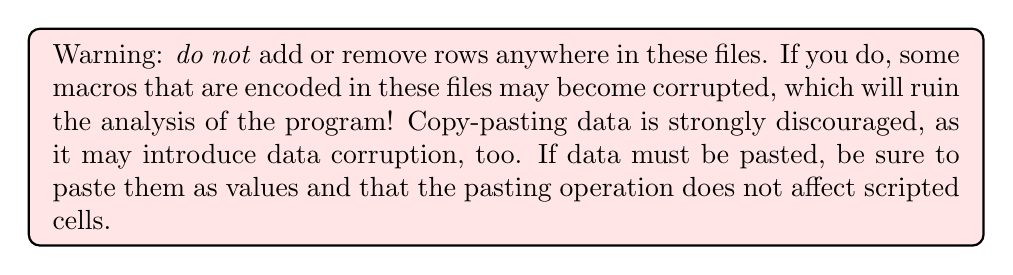
\begin{tikzpicture}
\node [minimum width = \textwidth, rounded corners, draw, thick, fill =
	red!10!white, align = justify, text width = 0.95\textwidth, inner
	sep = 0.2cm]
{Warning: \emph{do not} add or remove rows anywhere in these files. If you
	do, some macros that are encoded in these files may become
	corrupted, which will ruin the analysis of the program! Copy-pasting
	data is strongly discouraged, as it may introduce data corruption,
	too. If data must be pasted, be sure to paste them as values and
	that the pasting operation does not affect scripted cells.};
\end{tikzpicture}
\end{centering}

The template \texttt{.xlsx} has the following colors-scheme:
%
\begin{description}
	\item[gray:] parts that are comments or indications, do not edit
		these;
	\item[pink:] parts that are required (i.e., if you don't fill
		them then you won't get results); 
	\item[yellow:] parts that are optional, but recommended (i.e., if
		you don't fill them then you will get only partial results,
		and not everything that the tool may give you); 
	\item[green:] parts that you should fill if you want to get all the
		results that the suite can compute.
\end{description}
%
Thus: one should fill up at least all the pink parts. Doing the yellow and
green ones will produce more informative results (but of course will also
require more compilation time).


\subsubsection{The course summary sheet}
\label{sssec:the_course_summary_sheet}

The first sheet, called \texttt{course summary}, is a summary of the course and has the following information:

\begin{itemize}

	\itemheader{Prerequisite \acp{KC}}, which is a list of the \acp{KC}
		that are prerequisites for the course, i.e. \acp{KC} that
		students should be familiar with at the beginning of the
		course. See
		Section~\ref{sec:how_to_define_the_knowledge_components_list}
		for a description on how to identify these \acp{KC}. The
		\acp{KCM} supports up to 20 \acp{KC};
	
	\itemheader{Developed \acp{KC}}, which is a list of the \acp{KC}
		that the students should get familiar with as they advance
		through the course.
	
	\itemheader{\acp{TLA}}, which is a list of teaching and learning
		activities (lectures, classes, labs etc.) that occur in the
		course. See Section~\ref{sec:how_to_identify_tla} for a
		description on how to identify these \acp{TLA};
	
	\itemheader{\acp{ILO}}, which is a list of \acp{KC} that the
		students should have acquired after passing the course. See
		Section~\ref{sec:how_to_identify_ilo} for a description on
		how to identify these \acp{ILO};
	
	\itemheader{Starting and ending dates}, which are the dates when the
		course begins and ends, respectively. \textbf{Respect the
		format that is indicated in the \texttt{.xlsx} file};
	
	\itemheader{Taxonomy types}, which is a list of which taxonomy
		types, e.g., ``SOLO'' or ``Bloom'', that are included in
		this \ac{KCM}. If left blank, it defaults to ``SOLO''. See
		Section~\ref{sec:how_to_interpret_and_assign_taxonomy_levels}
		for a description of how to interpret and assign taxonomy
		levels;
	
	\itemheader{Course code}, which is self-explaining. If using a local
		repository, the file name should be equal to this entry.

\end{itemize}


\subsubsection{The developed vs.\ prerequisite KCs sheet}

The second sheet, called ``developed vs.\ prerequisite KCs'', is a
dependency matrix for the developed \acp{KC} versus the prerequisite
\acp{KC} and the developed \acp{KC}. In this matrix, each row is associated
with one of the \acp{KC} that are being developed in the course, and each
column is associated to either a prerequisite \ac{KC} or a developed
\ac{KC}. Assume that \texttt{X} is the row \ac{KC}, and \texttt{Y} is the
column \ac{KC}. Then the content of the cell \texttt{X-Y} shall indicate the
minimum taxonomical knowledge level that the students should have reached
about \texttt{Y} before starting learning \texttt{X} so to be able to learn
\texttt{X} in a satisfactory way. In other words, each entry says how much
(in a taxonomical knowledge way) the column \ac{KC} is instrumental to learn
the row \ac{KC}.

Note that if you did not fill up all 20 slots for the \acp{KC} in the
\texttt{course summary} tab then some rows and/or columns will show a ''0''
in the corresponding cell. This is a result of referencing a blank cell.


\subsubsection{The info on the developed KCs sheet}

The third sheet is a table of the developed \acp{KC} and has the following
information:

\begin{itemize}

	\itemheader{Developed \acp{KC}}, which is the same as in the course
		summary;
	
	\itemheader{Target taxonomy level}, which is the taxonomy level that
		the associated \ac{KC} should be known at by the end of the
		course;
	
	\itemheader{Time spent teaching}, which is the number of hours the
		course invests in teaching the associated \ac{KC};
	
	\itemheader{First lesson}, which is the number of the first teaching
		event when the associated \ac{KC} is taught.

\end{itemize}


\subsubsection{The remaining sheets}

The fourth sheet, called ``KCs vs.\ TLAs'', is similar to the second sheet
in the sense that it also is a dependency matrix. However, the meaning of
the rows and columns indexes is slightly different than before, and
indicates only a \emph{relation}: assume that \texttt{X} is the row
\ac{TLA}, and \texttt{Y} is the column \ac{KC}. Then a nonzero content in
the cell \texttt{X-Y} indicates that \texttt{Y} is either rehearsed or
taught during \texttt{X}. Moreover, the indicated taxonomical knowledge
level indicates at which complexity that rehearsal or teaching happens. In
other words, each entry says how much (in a taxonomical knowledge way) the
column \ac{KC} is rehearsed or taught during the row \ac{TLA}.

The fifth sheet, called ``info on the TLAs'', is similar to the third sheet,
but has information on the \acp{TLA} rather than \acp{KC}. This sheet holds
the following information:

\begin{itemize}

	\itemheader{\ac{TLA}}, which is the same as in the course summary;
	
	\itemheader{Time spent on activity}, which is the number of hours
		this course spends on the associated \ac{TLA};
	
	\itemheader{When the \ac{TLA} starts}, which is the number of the
		teaching event when the course starts hosting the associated
		\ac{TLA};
	
	\itemheader{When the \ac{TLA} ends}, which is the number of the
		teaching event when the course stops hosting the associated
		\ac{TLA}.

\end{itemize}

The sixth sheet, called ``developed KCs vs.\ ILOs'', is equivalent to the
fourth sheet. This time, though, each entry says how much (in a taxonomical
knowledge way) the column \ac{KC} is needed to reach the row \ac{ILO}.

\subsection{Summary of the procedure}

To summarize, to create a database that can be analysed through the COnCUR
one should follow these macro-steps:

\begin{enumerate}

	\itemheader{Create the program definition file}. This text document
		holds course codes, version numbers and links to these
		\acp{KCM} if they are on the Internet.
	
	\itemheader{Place the \acp{KCM} in the correct location}. If
		downloading the files over Internet, ensure that the links
		in the program definition file point to the correct URLs. If
		using a local repository, ensure that the \acp{KCM} are
		placed in the correct folder and named correctly.

\end{enumerate}

